\section{Conceptos previos}
En este apartado se describe la arquitectura de VMware Cloud Foundation, como estructura sus componentes internamente y cuales son los requisitos mínimos para realizar el despliegue de la plataforma\footnote{Se describen solo aquellos componentes que se utilizarán en el despliegue de Cloud Foundation.}.

%%%%%%%%%%%%%%%%%%%%%%%%%%%%%%
\iffalse
En este apartado se explican aquellos conceptos de VMware Cloud Foundation necesarios para entender su funcionamiento, configuración y requisitos de la infraestructura previos al despliegue del servicio.
\fi
%%%%%%%%%%%%%%%%%%%%%%%%%%%%%%%%


%% Workload Ddomains %&%&%%%%
%%%%%%%%%%%%%%%%%%%%%%%%%%%%
\subsection{Workload Domain}
Un \textit{workload domain} consiste en una instancia lógica de un SDDC que abarca todos o parte de los recursos de uno o más clusters, cuya función es aislar el flujo de trabajo de un usuario, aplicación o un determinado tipo de tareas. Cada \textit{workload domain} se extiende sobre varios hosts y contiene su propia instancia de vCenter Server, vSAN y NSX, lo cual permite establecer políticas de control únicas para todos los \textit{workload domains} y específicas para cada uno de ellos a la vez que se simplifica la complejidad de la infraestructura. Existen \underline{tres tipos} de \textit{workload domains} que permiten aislar las tareas de gestión de la infraestructura del resto de flujos de trabajo. 

%% MANAGEMENT DOMAIN
\subsubsection{Management Domain}
\label{subsubsec:domainManagement}
Este \textit{workload domain} se crea y configura automáticamente durante el proceso de despliegue de una instancia de VMware Cloud Foundation. Su función es gestión de todos los componentes de VMware Cloud Foundation, de toda la infraestructura y del resto de \textit{workload domains} existentes en el entorno a tráves de políticas establecidas desde un único punto. Los componentes dedicados a este \textit{workload domain} son SDDC Manager, vCenter Server, dos Platform Services Controllers que son redundantes, vRealize Log Insight y un vSwitch Distributed [Fig. \ref{fig:esquemaCFComponentes}]. Este dominio precisa los siguientes \underline{requisitos mínimos de hardware}:
\begin{itemize}
    \item \textbf{Hosts}: 4
    \item \textbf{CPU} por host: Dual-socket con 8 cores por socket, en sistemas All-Flash.
    \item \textbf{Memoria} total: 192 GB
    \item \textbf{Almacenamiento} por host: 16 GB para el dispositivo de arranque, un NVMe o SSD para la capa de caché, dos SSD o HDD para la capa de capacidad\footnote{En total se requieren 800 GB para este \textit{workload domain}.}.
    \item \textbf{NICs} por host: Dos NICs de al menos 10 GbE y, opcionalmente un NIC 1GbE BMC.
\end{itemize}

Cuando se \underline{despliega Management Domain se crean y configuran} de forma automatizada por SDDC Manager las siguientes máquinas virtuales (VM) de cada componente de Cloud Foundation:
\begin{itemize}
    \item Una VM de \textbf{SDDC Manager}: 4 vCPU, 16 GB de memoria, 800 GB de almacenamiento.
    \item Una VM de \textbf{vCenter Server}: 4 vCPU, 16 GB de memoria, 290 GB de almacenamiento.
    \item Dos instancias de \textbf{Platform Services Controller} (cada una): 2 vCPU, 4 GB de memoria, 60 GB de almacenamiento.
    \item Una VM de \textbf{NSX Manager}: 4 vCPU, 16 GB de memoria, 60 GB de almacenamiento.
    \item Tres VM de \textbf{NSX Controller} (cada una): 4 vCPU, 4 GB de memoria, 28 GB de almacenamiento.
    \item Tres VM de \textbf{vRealize Log Insight}, una en cada nodo: 8 vCPU, 16 GB de memoria, 1312 GB de almacenamiento.
\end{itemize}


%% VIRTUAL INF. DOMAIN
\subsubsection{Virtual Infrastructure Domain (VI) y Virtual Desktop Infrastructure Domain (VDI)}
\label{subsubsec:domainVI}
Este tipo de \textit{workload domain} se crea manualmente y bajo demanda desde el \textit{management domain} para dar servicio a las necesidades de cada usuario o para crear diferentes entornos con finalidades distintas. Su configuración de hardware y lógica se especifican durante su proceso de creación, permitiendo indicar la cantidad de hosts, cantidad de almacenamiento, políticas de rendimiento y disponibilidad, o configuración de la red disponibilidad, todo para satisfacer las necesidades de los usuarios que realizarán sus trabajos en él. El acceso a un \textit{VI domain} se realiza a través de vSphere Client donde su administrador puede gestionar todos los recursos asociados con ese \textit{workload domain}. Cada Virtual Infrastructure Domain cuenta con sus propios vCenter Server y un NSX Manager dedicados, que se ejecutan desde el \textit{management domain} de la infraestructura, y \textit{datastore} vSAN dedicado [Fig. \ref{fig:esquemaCFComponentes}]. La diferencia entre un \textit{virtual infrastructure domain} y \textit{virtual desktop infrastructure domain} es que el segundo incorpora el producto VMware Horizon View que, resumiendo, permite desplegar escritorios virtuales.\\
Un \textit{virtual infrastructure domain} precisa los siguientes \underline{requisitos mínimos de hardware}:
\begin{itemize}
    \item \textbf{Hosts}: 3
    \item \textbf{CPU}, \textbf{Memoria} y \textbf{Almacenamiento}: depende de los requisitos de las tareas que se vayan a desarrollar en este \textit{workload domain}.
    \item \textbf{NICs} por servidor: Dos NICs de al menos 10 GbE y, opcionalmente un NIC 1 GbE BMC.
\end{itemize}

Cuando se \underline{despliega un \textit{virtual infrastructure domain} se crean y configuran} de forma automatizada por el componente SDDC Manager las siguientes máquinas virtuales (VM) de cada componente de VMware Cloud Foundation:
\begin{itemize}
    \item Una VM de \textbf{vCenter Server} en Management Domain: 8 vCPU, 24 GB de memoria, 500 GB de almacenamiento.
    \item Una VM de \textbf{NSX Manager} en Management Domain: 4 vCPU, 16 GB de memoria, 60 GB de almacenamiento.
    \item Tres VM de \textbf{NSX Controller} en el VI Domain creado (cada una):  4 vCPU, 4 GB de memoria, 28 GB de almacenamiento.
\end{itemize}

En total, si la infraestructura cuenta con un Management Domain y al menos un Virtual Infraestructure Domain, entonces se necesita una \setword{capacidad}{Word:capacidad} inicial y como mínimo igual a 76 vCPU, 168 GB de Memoria y 3306 GB de almacenamiento.

\begin{figure}[h!]
  \centering
  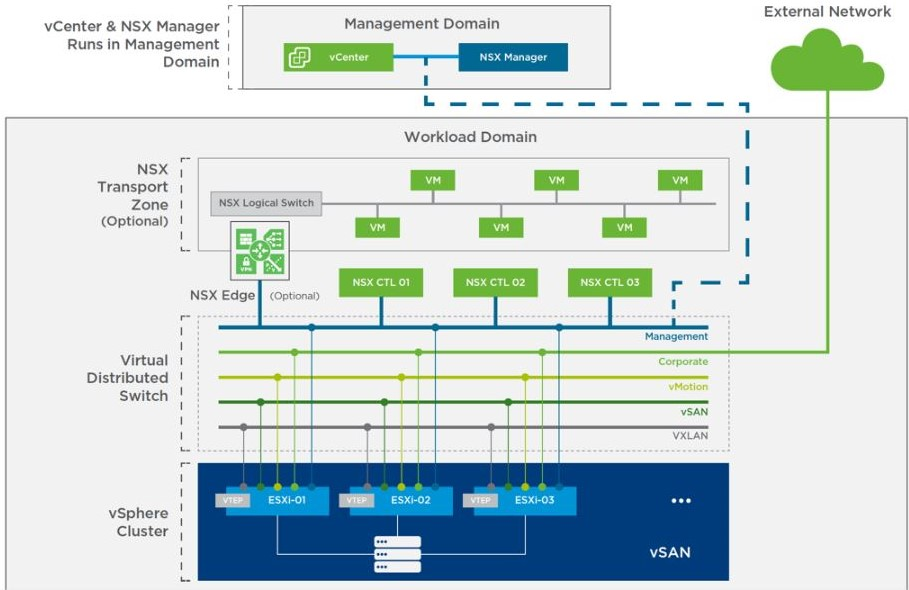
\includegraphics[width=1\textwidth]{imaxes/conceptosPrevios/WDomainStructure.JPG}
  \caption{Como se estructuran y conectan los componentes de VMware Cloud Foundation.}
  \label{fig:esquemaCFDominios}
\end{figure}
\begin{figure}[h!]
  \centering
  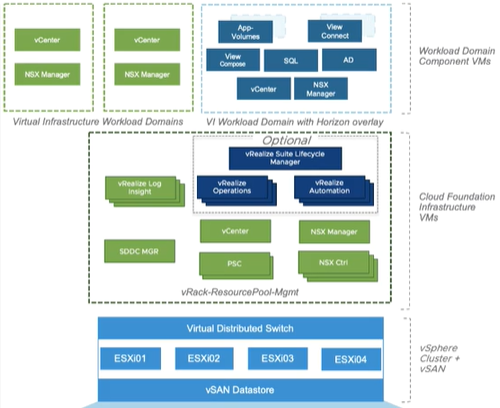
\includegraphics[width=1\textwidth]{imaxes/conceptosPrevios/workloadDomains.png}
  \caption{Componentes dedicados de cada \textit{workload domain}.}
  \label{fig:esquemaCFComponentes}
\end{figure}
\FloatBarrier

%&%%%%%%%%%%%%%%%%%%%%%%%%%%%%%%%%%%%%%%%%%%%%%%%%%%%%%%%%
%% ARQUITECTURA
\subsection{Arquitectura}
La arquitectura de VMware Cloud Foundation tiene dos posibles modelos de despliegue dependiendo del número de hosts sobre los que se despliega VMware Cloud Foundation.

%% ESTANDAR
\subsubsection{Modelo estándar}
Este modelo se utiliza cuando VMware Cloud Foundation se despliega en un entorno con siete o más hosts. Está formado por un \underline{management domain} que se despliega en uno de los hosts y que contiene todos los componentes de gestión de toda la infraestructura [Sec. \ref{subsubsec:domainManagement}], y por \underline{virtual infrastructure domains} que se crean bajo demanda sobre el resto hosts disponibles [Sec. \ref{subsubsec:domainVI}] y una vez creado se pueden ampliar o reducir sus capacidades según sea necesario. El máximo número de \underline{virtual infrastructure domains} que se pueden desplegar en una instacia de VMware Cloud Foundation es 15.

\begin{figure}[h!]
  \centering
  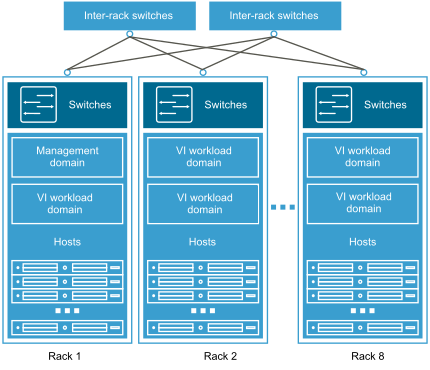
\includegraphics[width=0.75\textwidth]{imaxes/conceptosPrevios/arquitect_standarCF.png}
  \caption{Esquema del modelo de arquitectura estándar.}
  \label{fig:modelostandard}
\end{figure}

\begin{figure}[h!]
  \centering
  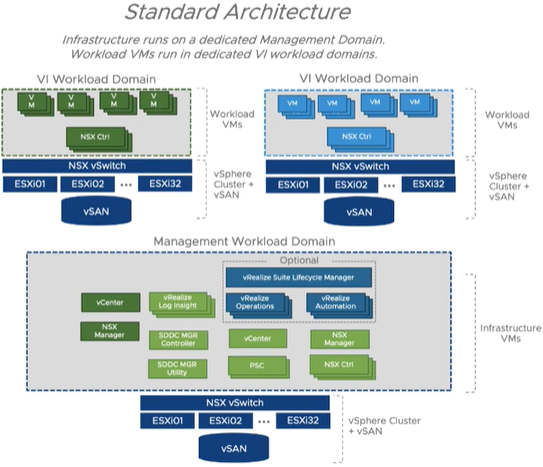
\includegraphics[width=0.85\textwidth]{imaxes/conceptosPrevios/standardArch.png}
  \caption{Estructura de los componentes en una arquitectura estándar.}
  \label{fig:standardarch}
\end{figure}
\FloatBarrier
%%%%%%%%%%%%%%%%%%%%%
%%  CONOLIDADO
\subsubsection{Modelo consolidado}
Este modelo se despliega cuando el entorno esta formado por menos de siete nodos. En este modelo el flujo de trabajo que corresponde al \underline{virtual infrastructure domain} y al \textit{management domain} en el despliegue estándar, está colocado dentro del mismo \underline{workload domain}, es decir, solo existe un único \textit{workload domain} denominado \textit{management domain}. Este modelo se puede convertir en un modelo estándar creando un \textit{virtual infrastructure domain}. Los flujos de trabajo se mantienen aislados gracias a sus respectivos almacenes de recursos[Fig. \ref{fig:modeloconsolidated}].

\begin{figure}[h!]
  \centering
  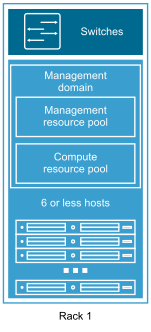
\includegraphics[width=0.25\textwidth]{imaxes/conceptosPrevios/modelConsolidated.png}
  \caption{Esquema del modelo de arquitectura consolidado.}
  \label{fig:modeloconsolidated}
\end{figure}

\begin{figure}[h!]
  \centering
  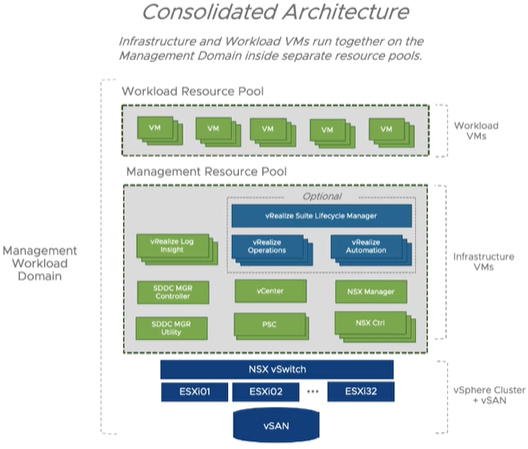
\includegraphics[width=0.85\textwidth]{imaxes/conceptosPrevios/consolidatedArch.png}
  \caption{Estructura de los componentes de una arquitectura consolidado.}
  \label{fig:consolidatedArch}
\end{figure}
\FloatBarrier

%%% CLOUD BUILDER
\subsection{Cloud Foundation Builder VM Support}
\label{subsec:cloudBuilder}
El despliegue de la plataforma VMware Cloud Foundation se realiza través de una máquina virtual llamada Cloud Foundation Builder. Esta máquina recoge la configuración que se indica en la hoja de parámetros, los valida, , despliega y configura el \underline{Management Domain}. Al final del proceso, transfiere el inventario y el control del sistema al componente SDDC Manager y esta máquina virtual puede ser eliminada.\\
\underline{Requisitos mínimos} de VMware Cloud Foundation Builder VM:
\begin{itemize}
    \item \textbf{CPU}: 4vCPUs
    \item \textbf{Memoria}: 4 GB
    \item \textbf{Almacenamiento}: 350 GB
    \item \textbf{Conectividad}: acceso a la red de gestión para acceder a cada nodo, al servidor DNS y al servidor NTP.
\end{itemize}

\subsection{Red, almacenamiento y servicios necesarios para el despliegue}

\subsubsection{Servicios internos}
\label{subsubsec:servInterno}
Durante el despliegue Cloud Foundation, hay servicios y puertos deben estar habilitados en cada nodo ESXi para Cloud Foundation Builder (Fig. \ref{fig:puertosCB}) y SDDC Manager (Fig. \ref{fig:puertosSDDC}) puedan acceder a todos los componentes.
\iffalse
\begin{figure}[h!]
  \centering
  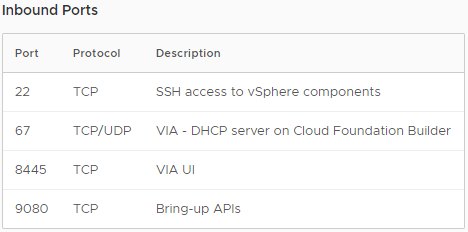
\includegraphics[width=0.7\textwidth]{imaxes/conceptosPrevios/puertosentradaCB.png}
  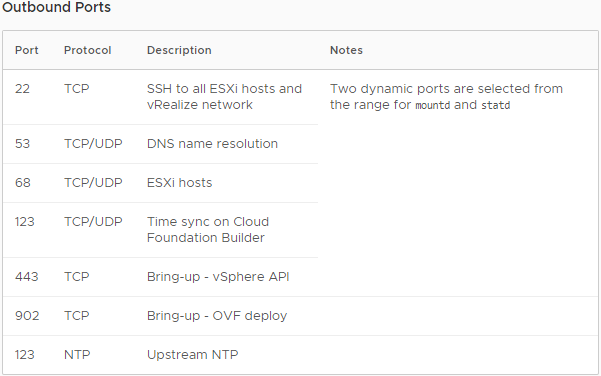
\includegraphics[width=0.7\textwidth]{imaxes/conceptosPrevios/puertossalidaCB.png}
  \caption{Servicios y puertos de entrada y salida habilitados para Cloud Foundation Builder.}
  \label{fig:puertosCB}
\end{figure}

\begin{figure}[h!]
  \centering
  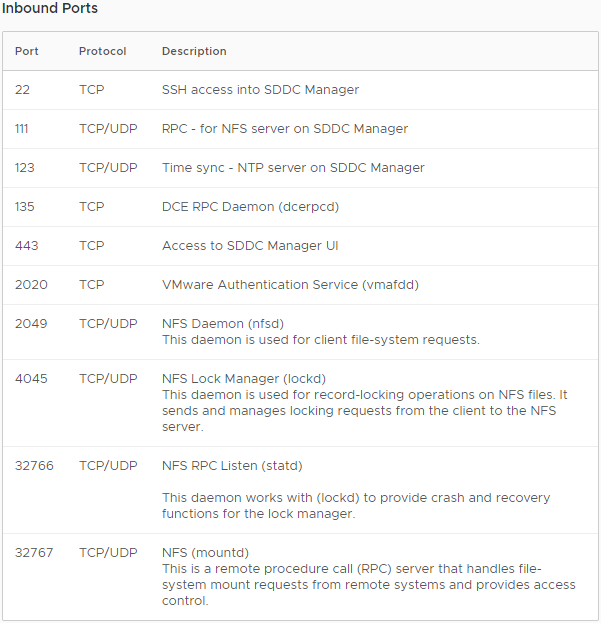
\includegraphics[width=0.7\textwidth]{imaxes/conceptosPrevios/puertosentradaSDDC.png}
  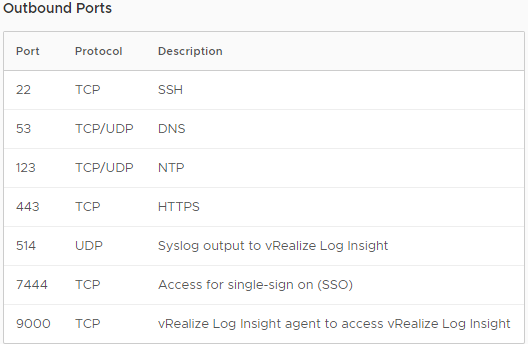
\includegraphics[width=0.7\textwidth]{imaxes/conceptosPrevios/puertossalidaSDDC.png}
  \caption{Servicios y puertos de entrada y salida habilitados para SDDC Manager.}
  \label{fig:puertosSDDC}
\end{figure}
\fi

\begin{figure}[h!]
  \centering
  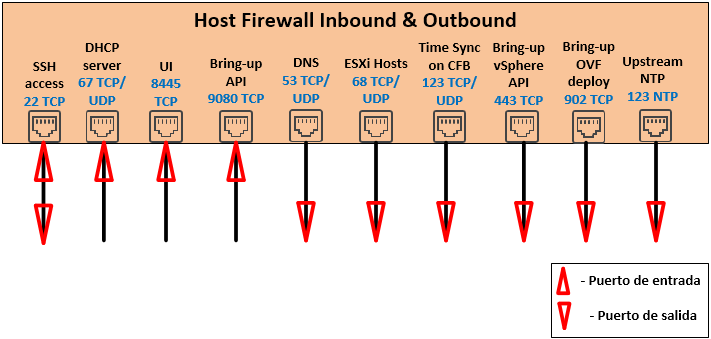
\includegraphics[width=1\textwidth]{imaxes/conceptosPrevios/firewall_CloudBuilder.png}
  \caption{Servicios y puertos de entrada y salida habilitados para Cloud Foundation Builder.}
  \label{fig:puertosCB}
\end{figure}
\begin{figure}[h!]
  \centering
  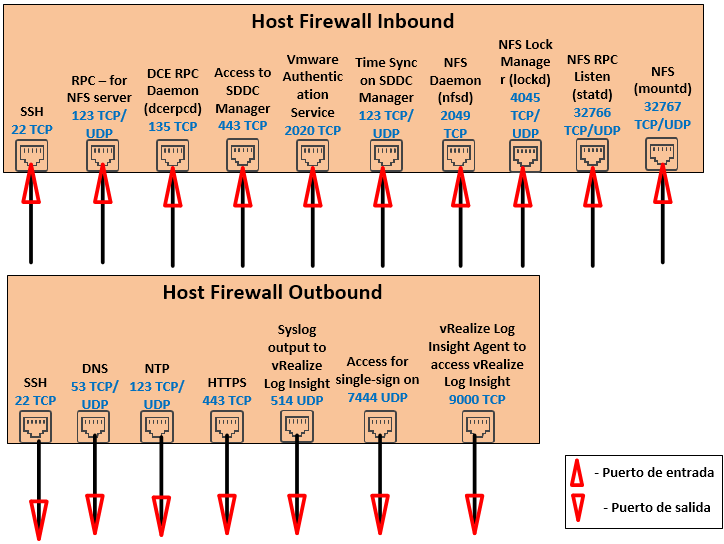
\includegraphics[width=1\textwidth]{imaxes/conceptosPrevios/firewall_SDDC.png}
  \caption{Servicios y puertos de entrada y salida habilitados para SDDC Manager.}
  \label{fig:puertosSDDC}
\end{figure}

%%%%%%%%%%%%%%%%%%%%%%%%%%%%%%%%%%%%%%%%%%%%%%%%%%%%%%%%%%%%%%%%%%%%%%%%
\iffalse
\begin{itemize}
\item Cloud Builder:
    \begin{itemize}
        \item Entrada:
            \begin{itemize}
                \item SSH: 22, TCP
                \item VIA - Servidor DHCP en Cloud Foundation Builder: 67, TCP/UDP
                \item VIA - Interfaz de Usuario: 8445, TCP
                \item APIs para controlar los componentes: 9080, TCP
            \end{itemize}
        \item Salida:
            \begin{itemize}
                \item SSH: 22, TCP
                \item DNS: 53, TCP/UDP
                \item Hosts ESXi: 68, TCP/UDP
                \item NTP: 123, TCP/UDP
                \item API para iniciar vSphere: 443, TCP
                \item Despliegue de archivos OVF: 902, TCP
            \end{itemize}
    \end{itemize}
\item SDDC Manager:
        \begin{itemize}
        \item Entrada:
            \begin{itemize}
                \item SSH: 22, TCP
                \item RPC para servidor NFS: 111, TCP/UDP
                \item NTP: 123, TCP/UDP
                \item DCE RPC: 135, TCP
                \item Interfaz de Usuario: 443, TCP
                \item Servicio de Autenticación: 2020, TCP
                \item Demonio NFS (nfsd): 2049, TCP/UDP
                \item NFS Lock Manager (lockd): 4045, TCP/UDP
                \item NFS RPC (statd): 32766, TCP/UDP
                \item NFS (mountd): 32767 , TCP/UDP
            \end{itemize}
        \item Salida:
            \begin{itemize}
                \item SSH: 22, TCP
                \item DNS: 53, TCP/UDP
                \item HTTPS: 443, TCP
                \item NTP: 123, TCP/UDP
                \item Syslog hacia vRealize Log Insight: 514, UDP
                \item Acceso Single-Sign On: 7444, TCP
                \item Agente vRealize Log Insight: 9000, TCP
            \end{itemize}
    \end{itemize}
\end{itemize}
\fi

%%%%%%%%%%%%%%%%%%%%%%%%%%%%%%%%%%%%%%%%%%%%%%%%%%%%%%%%%%%%%%%%%%%%%%%%%%%%%
\FloatBarrier

\subsubsection{Servicios externos}
\label{subsubsec:servExterno}
En este apartado se describen aquellos servicios necesarios para el despliegue de VMware Cloud Foundation
\begin{itemize}
    \item \textbf{Dynamic Host Configuration Protocol (DHCP)}: Permite configurar automáticamente cada puerto VMkernel de un nodo con IPv4. 
    \item \textbf{Domain Name Server (DNS)}: Un servidor DNS debe estar disponible para todos los componentes desde el momento de despliegue. También se debe especificar el nombre del dominio. Con esto los componentes pueden obtener tanto el nombre como la dirección IP de un elemento en la red. NTP, Platform Services Controller, instancias de vCenter Server, instancias de NSX Manager, vRealize Log Insight.
    \item \textbf{Network Time Protocol (NTP)}: Permite la sincronizar el tiempo en todos los nodos de la infraestructura. Durante el despliegue se debe especificar la dirección IP de al menos un servidor NTP.
\end{itemize}
Se puede encontrar más información sobre otros servicios opcionales en el siguiente \href{https://docs.vmware.com/en/VMware-Cloud-Foundation/3.9/com.vmware.vcf.planprep.doc_39/GUID-F022BD3C-F11C-4EE6-83EA-ABE016E7A9B9.htm}{enlace}.
\FloatBarrier

%%%%% RED 
\subsubsection{Red física}
\label{subsubsec:redFisica}
La red física debe admitir las siguientes características:
\begin{itemize}
    \item \textbf{VLAN}: etiquetado de redes VLAN (802.1Q)
    \item \textbf{Jumbo Frames}: MTU mínimo igual a 1600, aunque se recomienda que sea igual a 9000.
\end{itemize}

\subsubsection{Red lógica}
\label{subsubsec:redLogicaCF}
Antes del despliegue es necesario especificar varias redes que más tarde Cloud Foundation usará para automatizar la configuración de puertos \ref{Word:vmkernel} cuando se añade un nuevo host al entorno o se crea un VI Domain. Estas redes son  una dedicada al servicio \underline{vSAN}, otra dedicada a \underline{vMotion}, ota de dedicada a la gestión de los componentes y otra dedicada al tráfico de las máquinas virtuales. Los datos a especificar son la etiqueta VLAN, MTU, IP de la red, máscara, gateway y el rango de direcciones IP. Una vez creadas solo se puede modificar el rango de direcciones IP.\\
Es importante utilizar VLANs e IPs ya que es en lo que se basa Cloud Foundation para aislar cada tipo de tráfico de la infraestructura. La cantidad de subredes necesarias depende del número de Workload Domains que se creen, número de clusters y otros componentes opcionales.

\subsubsection{Almacenamiento}
Según la documentación de vSAN, cada host ESXi del entorno debe tener como mínimo un grupo de discos. Un nodo puede tener hasta cinco grupos de discos, dentro de los cuales debe haber al menos un disco de caché y un disco de capacidad. Cada grupo de discos puede contener hasta siete discos de capacidad.
En cuanto al tipo de disco que se debe utilizar, los discos de caché deben ser SSD y los discos de capacidad pueden ser SSD o HDD, según el modelo que se quiera implementar (All-Flash o híbrido).

%%%%%%%%%%%%%%%%%%%%%%%%%%%%%%%%%%%%%%%

\iffalse
\subsection{Nombres y direcciones IP}
Cloud Foundation requiere especificar el nombre que se le da a cada componente y su r
Durante el despliegue hay que especificar el nombre de cada componente y su dirección IP. Estos componentes son los servicios externos, los componentes internos de Cloud Foundation como SDDC Manager, Platform Services Controller, vCenter Server, cada nodo ESXi, cada instancia de NSX y de vRealze Log Insight.
\fi


\iffalse
a
\subsection{Instancias de los componentes}
Para cada workload domain que se crea, SDDC Manager genera una serie de instancias de cada componente tanto en Management Domain como en cada Virtual Infraestructure Domain. Estas instancias son:
\subsubsection{Management Domain}
Una instancia de vCenter Server. Para la gestión de la red de este dominio, despliega una instancia de NSX Manager(centraliza la gestión de la red, aporta APIs para crear configurar y monitorizar cada componente de NSX como los switches lógicos o los servicios que operan en el gateway de salida de la red) y tres instancias de NSX Controller (gestiona el vSwitch distribuído y el enrutamiento del tráfico, controlando todos los vswitches de la red y manteniendo información sobre todas las VM, nodos, vSwitches y VXLANs. Para la gestiión de logs, se instala 
\fi
